\section{Conceptual models of Experimentation on SE}\label{sec:annex-models-SE}

\odnote{Me temo que tendremos que traducir los modelos a ingl�s. Aunque sea un trabajo extra, no nos queda m�s remedio porque los vamos a necesitar para la discusi�n del paper de la SLR. Si los publicamos aqu�, ya los tendremos disponibles.}

\begin{figure*}[htbp!]
	\centering
	\captionsetup{justification=centering}
	
\includegraphics[width=\textwidth]{images/Producto-Intermedio-Revision-Lit}
	\caption{Modelo conceptual preliminar resultado del an�lisis de la literatura relevante.}
	\label{fig-conceptos-preliminar}\odnote{RODRIGO: Poner modelo completo}.
\end{figure*}

\begin{figure*}[htbp!]
	\centering
	
\includegraphics[width=5in]{images/Producto-Final-Revision-Lit}
	\caption{Modelo conceptual resultado del an�lisis de los materiales experimentales.}
	\label{fig-conceptos-final-revision-fuentes}\odnote{RODRIGO: Poner modelo completo}.
\end{figure*}

\begin{figure*}[htbp!]
	\centering
	\includegraphics[width=5in]{images/Producto-Final-Observacion-Par}
	\caption{Modelo conceptual resultado de la observaci�n participativa.}
	\label{fig-conceptos-final-observacion-participativa}\odnote{RODRIGO: Hay que crear esta figura.}
\end{figure*}

\begin{figure*}[htbp!]
	\centering
	\includegraphics[width=5in]{images/Model}
	\caption{Modelo conceptual resultado de las entrevistas semi-estructuradas.}
	\label{fig-modelo-exp}\odnote{RODRIGO: Hay que crear esta figura.}
\end{figure*}

\begin{sidewaysfigure}%[htbp!]
	\centering
	\includegraphics[height=6in]{images/Final-Proccess-Workflow}
	\caption{Workflow del proceso de experimentaci�n en SE resultado de las entrevistas semi-estructuradas.}
	\label{fig-final-process-workflow}
\end{sidewaysfigure}

\begin{figure}[htbp!]
	\centering
	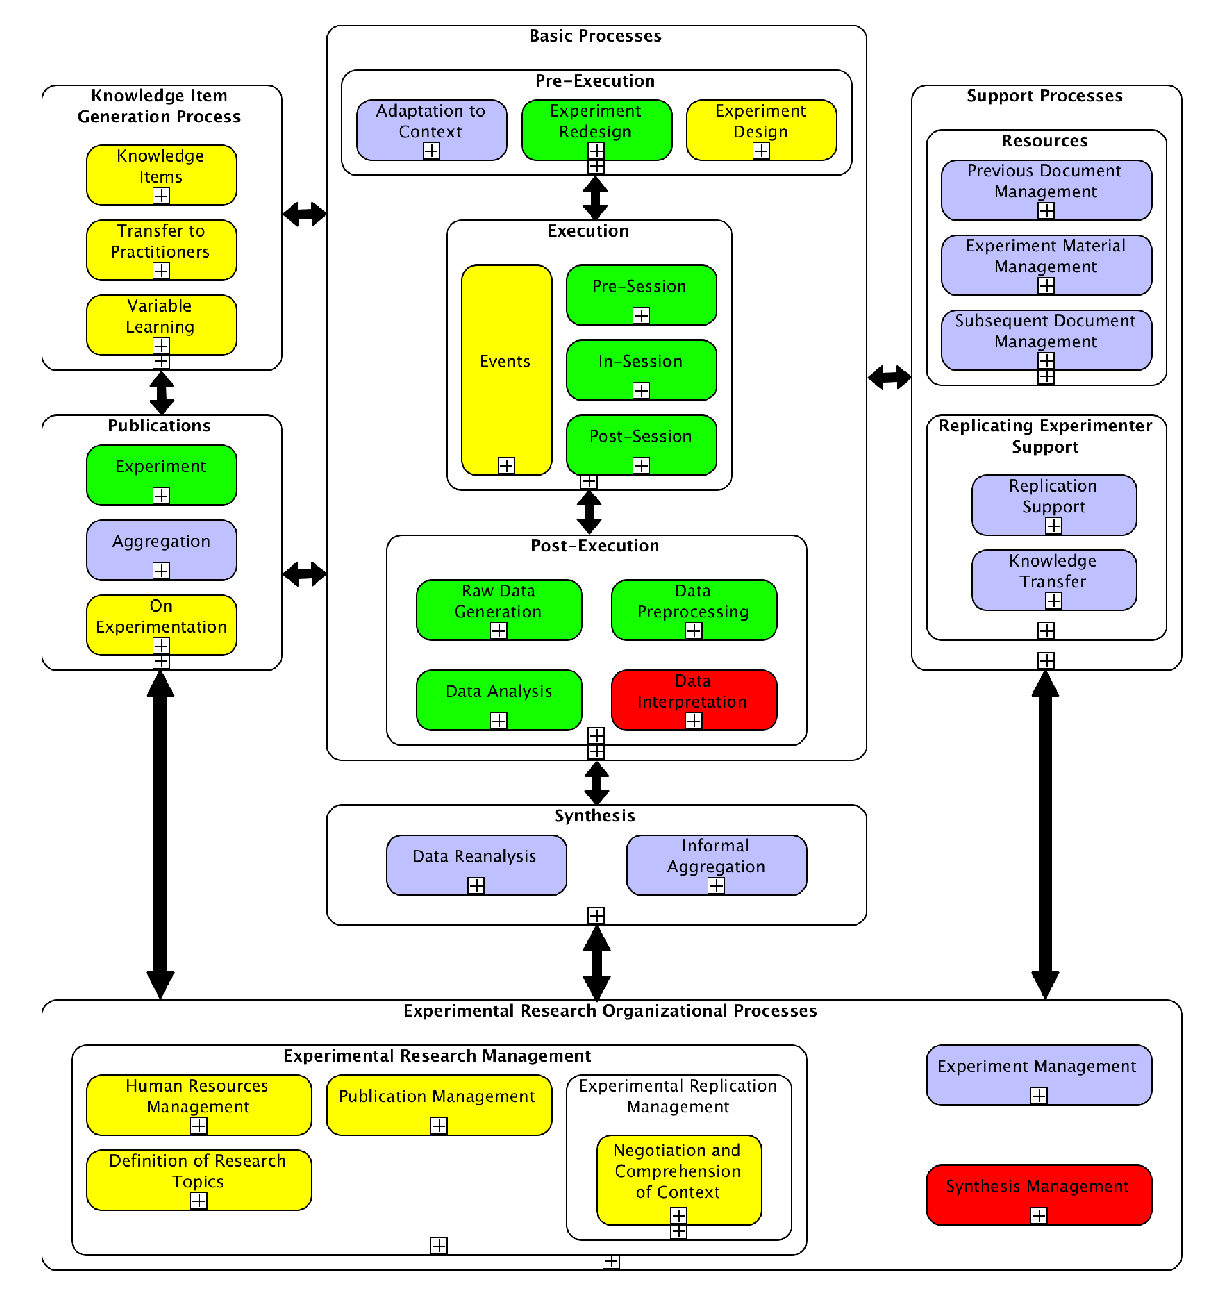
\includegraphics[height=6in]{Images/Final-Experimentation-Process-Model}
	\caption{Modelo del proceso de experimentaci�n en SE resultado de las entrevistas semi-estructuradas.}
	\label{fig-final-process-model}
\end{figure}

\begin{sidewaysfigure}%[htbp!]
	\centering
	\includegraphics[height=6in]{Images/Conceptual-Model-RM}
	\caption{SE Conceptual Model From Research Manager Point Of View}
	\label{fig-conceptual-model-RM}
\end{sidewaysfigure}

\begin{sidewaysfigure}%[htbp!]
	\centering
	\includegraphics[height=6in]{Images/Conceptual-Model-EM}
	\caption{SE Conceptual Model From Experiment Manager Point Of View}
	\label{fig-conceptual-model-EM}
\end{sidewaysfigure}

\begin{sidewaysfigure}%[htbp!]
	\centering
	\includegraphics[height=6in]{Images/Conceptual-Model-SE}
	\caption{SE Conceptual Model From Senior Experimenter Point Of View}
	\label{fig-conceptual-model-SE}
\end{sidewaysfigure}

\FloatBarrier

\section{Conceptual models of Experimentation on Biotechnology}\label{sec:annex-models-BIO}

\begin{figure}[htbp!]
	\centering
	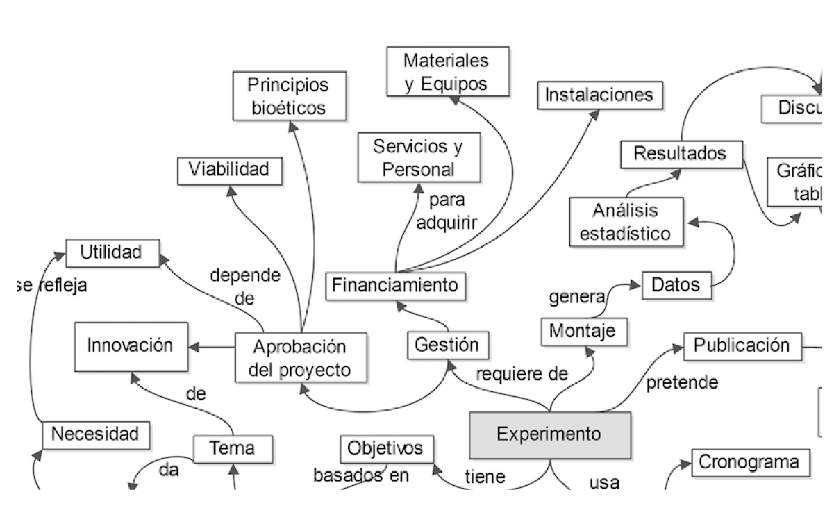
\includegraphics[width=3in]{Images/Concepts-Final-Bio}
	\caption{Modelo Conceptual final de experimentaci�n en Biotecnolog�a}
	\label{fig-concepts-final-bio}\odnote{RODRIGO: Poner modelo completo}.
\end{figure}

\begin{figure}[htbp!]
	\centering
	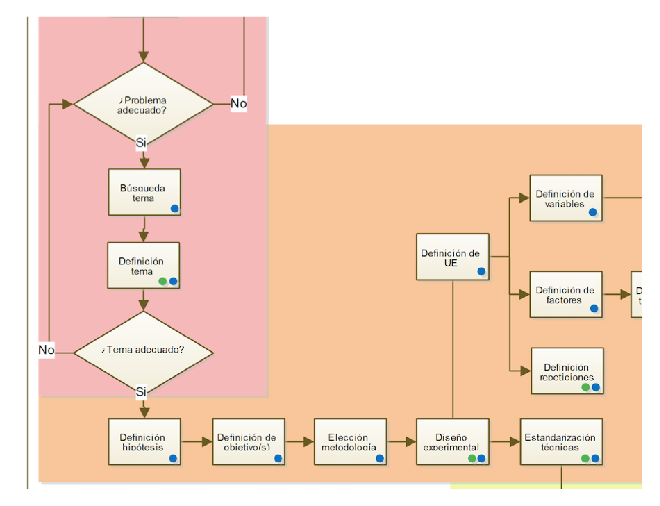
\includegraphics[width=3.2in]{Images/Final-Process}
	\caption{Modelo final del proceso experimental en Biotecnolog�a}
	\label{fig-proceso-exp-final}\odnote{RODRIGO: Poner modelo completo}.
\end{figure}